% !TEX root = ../main.tex
% SECTION 7: KUPPLUNGEN
% Inhalt: Liv Erne, Silvio Seiz — Form: ZSF-Template-Rework
% ============================================================

\StartChapter[ch:kupplungen]{Kupplungen}
\ZSFindex{Kupplung}

\ZSFfig[0.70]{graphics/v9_kupplungsbaum_entscheidungsbaum.png}{Kupplungsbaum}{}\begin{propertylist}[Eigenschaften]
\ZSFFact{Schaltbar}{Verbindung/Trennung des Drehmomentflusses}
\ZSFFact{Drehsteif}{Drehmomentstösse/Schwankungen gehen ungefiltert durch}
\ZSFFact{Drehelastisch}{Dämpfung von Stössen/Schwankungen (Gummi, Federn)}
\ZSFFact{Ausgleichend}{Ausgleich von Versatz:~axial ($\ZSFcoupDeltaKa$), radial ($\ZSFcoupDeltaKr$), winklig ($\ZSFcoupDeltaKw$)}
\ZSFFact{Fremdbetätigt}{Betätigung von aussen (manuell, hydr., el.)}
\ZSFFact{Selbstbetätigt}{Schaltet selbsttätig bei Grenzwert:\\
-- \textbf{Drehzahl}:~Schalten ab $\ZSFcoupNlimit$ (Fliehkraftkupplung)\\
-- \textbf{Moment}:~Rutschen bei Überlast $\ZSFcoupMlimit$ (Sicherheitsk.)\\
-- \textbf{Richtung}:~Freilauf / Sperrrichtung (Freilaufkupplung)}
\end{propertylist}

\SubsectionBarOnNewColumn[sec:fliehkraftkupplung]{Fliehkraftkupplung (drehzahlbetätigt)}
\ZSFindex{Fliehkraftkupplung}

\begin{splitbox}[0.45]
Durch die Drehbewegung werden die \ZSFkeyword[Fliehgewicht]{Fliehgewichte} im Inneren der Kupplung nach aussen gedrückt, wodurch ein Reibschluss mit der Kupplungsglocke entsteht. Die Berechnungen weichen, je nach Anzahl Fliehgewichte, ab: Gleichgewicht zwischen Federkraft $\ZSFcoupFF = \ZSFcoupFV$ und $\ZSFcoupFz$ aufstellen.
\tcblower
\centering
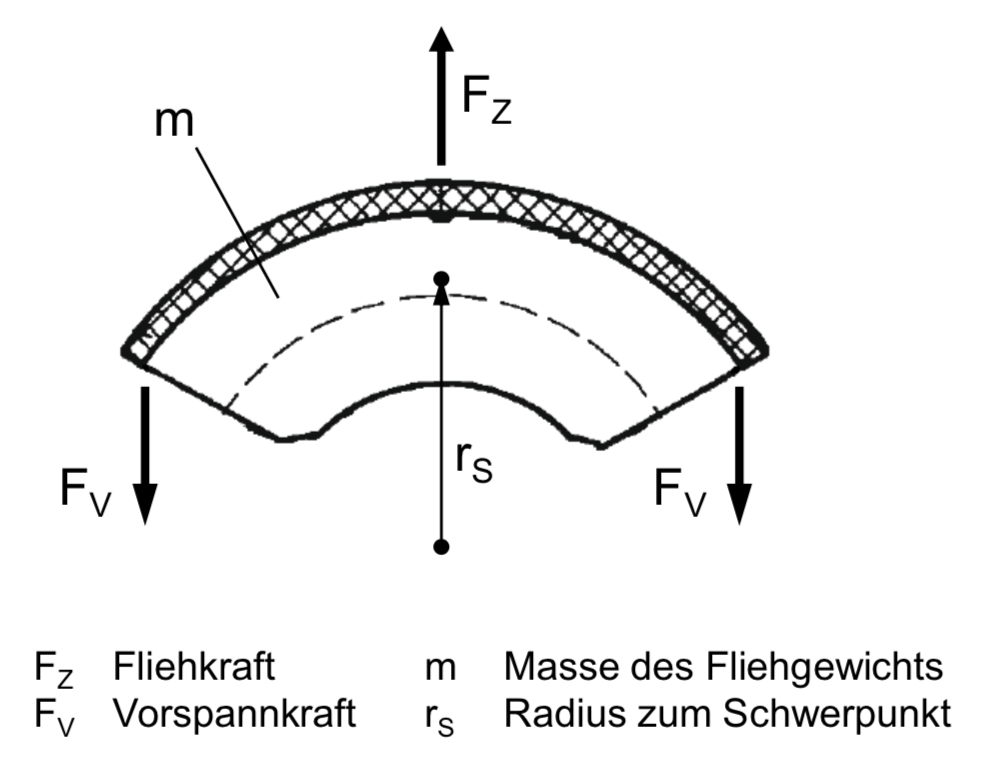
\includegraphics[width=\linewidth,keepaspectratio]{graphics/centrifugal_clutch_weight_forces.png}
\end{splitbox}
% Danger-Pill unbrechbar (~190pt) — passt nur in voller Spaltenbreite,
% deshalb direkt nach der splitbox statt in deren schmaler Textspalte.
\ZSFdanger{so kann es bei den Drehzahl Formeln auch sin oder cos drin haben}

\begin{formulabox}[Drehzahlen]
\formulasources{$\ZSFcoupFV$, $\ZSFcoupR$:~gegeben oder \ZSFsource{bestimmen mit}{sec:zugdruckfedern}}
\[ \ZSFcoupFz = \ZSFcoupNf\cdot \ZSFcoupFV = \dfrac {\ZSFcoupMass\cdot \ZSFcoupV^2}{\ZSFcoupRs} = \ZSFcoupMass\cdot \ZSFcoupRs \cdot (2\cdot \pi \cdot \ZSFcoupN)^2 = \dfrac{\ZSFcoupMass\cdot \ZSFcoupRs \cdot 4\cdot \pi^2}{\ZSFcoupT^2} \]
\[ \ZSFcoupNG^2 = \dfrac{\ZSFcoupNf\cdot \ZSFcoupFV}{\ZSFcoupMass\cdot \ZSFcoupRs \cdot 4\cdot \pi^2} \quad \text{\textbf{Grenzdrehzahl}} \]
\formulasep
\[ \ZSFcoupNE^2 = \dfrac{\ZSFcoupNf\cdot (\ZSFcoupFV + \ZSFcoupR\cdot \ZSFcoupApos)}{\ZSFcoupMass\cdot (\ZSFcoupRs + \ZSFcoupApos) \cdot 4\cdot \pi^2} \quad \text{\textbf{Einschaltdrehzahl}} \]
\[ \ZSFcoupNB^2 = \dfrac{\ZSFcoupFN + \ZSFcoupNf\cdot (\ZSFcoupFV + \ZSFcoupR\cdot \ZSFcoupApos)}{\ZSFcoupMass\cdot (\ZSFcoupRs + \ZSFcoupApos) \cdot 4\cdot \pi^2} \quad \text{\textbf{Betriebsdrehzahl}} \]
\formulanote{$\ZSFcoupN^2 = [s^{-2}]$, $\ZSFcoupN = [s^{-1}]\rightarrow\cdot 60 = \ZSFcoupN = [min^{-1}]$}
\[ \ZSFcoupFN = \dfrac{\ZSFcoupM}{\ZSFcoupZ\cdot \ZSFcoupMu \cdot \ZSFcoupRk} \]
\formulanote{$\ZSFcoupZ$:~Anzahl Fliehgewichte \ $\cdot$ \ $\ZSFcoupRk$:~wirksamer Reibradius}
\formulanote{$\ZSFcoupNf$:~Anzahl Federn pro Fliehgewicht \ $\cdot$ \ $\ZSFcoupR$:~Federrate}
\formulanote{\ZSFdanger{Achtung:} $2\cdot \ZSFcoupR\cdot \ZSFcoupApos$, anstelle $\ZSFcoupR\cdot \ZSFcoupApos$, falls der Weg a zweimal gemacht wird.}
\end{formulabox}
\ZSFindex{Grenzdrehzahl}
\ZSFindex{Einschaltdrehzahl}
\ZSFindex{Betriebsdrehzahl}

\SubsectionBar[sec:rutschkupplung]{Rutsch- o. Sicherheitskupplung (momentbetätigt)}
\ZSFindex{Rutschkupplung}
\ZSFindex{Sicherheitskupplung}

\begin{splitbox}[0.57]
\centering
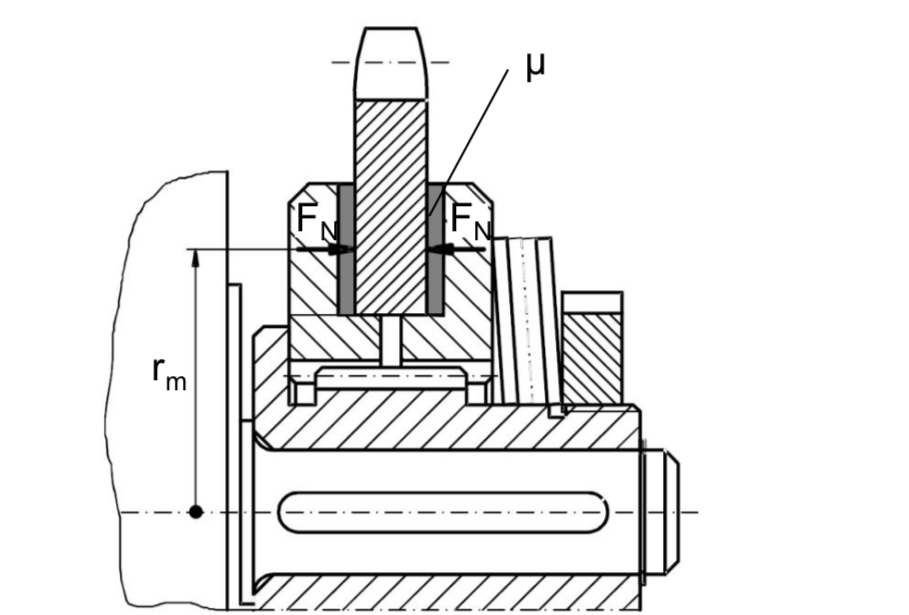
\includegraphics[width=\linewidth,keepaspectratio]{graphics/rutschkupplung_reibscheiben_normalkraft_reibwert.png}
\tcblower
\centering
$\begin{aligned}
\ZSFcoupFt &= \ZSFcoupZR\cdot \ZSFcoupFr \\[1pt]
\ZSFcoupFr &= \ZSFcoupMu \cdot \ZSFcoupFN \\[1pt]
\ZSFcoupRm &= \dfrac{\ZSFcoupDa + \ZSFcoupDi}{4} \\[1pt]
\ZSFcoupP &= \dfrac{\ZSFcoupFN}{\ZSFcoupAm} \\[1pt]
\ZSFcoupAm &= \dfrac{\pi}{4}\cdot (\ZSFcoupDa^2 - \ZSFcoupDi^2) \\[1pt]
\ZSFcoupFN &= \ZSFcoupNFedern \cdot \ZSFcoupFV
\end{aligned}$

\ZSFgapXS
{\ZSFfontNote $\ZSFcoupFV$:~Vorspannkraft einer Feder \ $\cdot$ \ $\ZSFcoupZR$:~Anzahl Reibflächen \\
$\ZSFcoupDa$:~Aussendurchmesser \ $\cdot$ \ $\ZSFcoupDi$:~Innendurchmesser\par}
\end{splitbox}

\begin{formulabox}[Grenzmoment $\ZSFcoupMG$]
\[ \ZSFcoupMG = \ZSFcoupFt \cdot \ZSFcoupRm = \ZSFcoupZR\cdot \ZSFcoupMuG \cdot \ZSFcoupFN \cdot \ZSFcoupRm \]
\formulanote{$\ZSFcoupMuG$:~Gleitreibwert \ $\cdot$ \ $\ZSFcoupZR$:~Anzahl Flächen oder Reibkontakte}
\end{formulabox}

\SubsectionBar[sec:nichtschaltbar]{Nicht schaltbare Kupplungen}
\ZSFindex{Kupplung!nicht schaltbar}

\begin{tablebox}[Nicht schaltbare Kupplungen: Drehsteif]
\ZSFKupplungenDrehsteifTabelle
\end{tablebox}

\begin{tablebox}[Nicht schaltbare Kupplungen: Drehelastisch]
\ZSFKupplungenDrehelastischTabelle
\end{tablebox}

\begin{tablebox}[Grosser Radialversatz / Winkelausgleich]
\setlength{\tabcolsep}{2.0pt}
\begin{ZSFtablePlain}[\ZSFfontTableDense]{Z{1.0} Z{1.0} Z{1.0}}
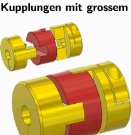
\includegraphics[height=0.7cm,keepaspectratio]{graphics/kreuzscheibenkupplung.png} &
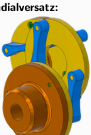
\includegraphics[height=0.7cm,keepaspectratio]{graphics/parallelkurbelkupplung.png} &
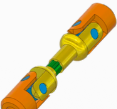
\includegraphics[height=0.7cm,keepaspectratio]{graphics/kardangelenkwelle.png} \\
\TableTitle{Kreuzscheiben\-kupplung} &
\TableTitle{Parallelkurbel\-kupplung} &
\TableTitle{Kardangelenkwelle}
\end{ZSFtablePlain}
\end{tablebox}
